\documentclass{hw}
\usepackage{mhchem}
\usepackage{nuc}
\usepackage[load=addn]{siunitx}
\usepackage{amsmath}
\usepackage{cancel}
\usepackage{physics}
\graphicspath{ {images/}}

\author{J.R. Powers-Luhn}
\date{2016/10/25}
\title{Homework No. 4}

\begin{document}

\problem{}
Consider a thin slab of $\ce{^{235}U}$ with the incident thermal neutron beams shown below: \\
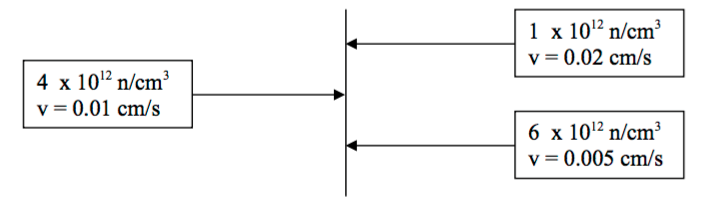
\includegraphics[width=5in,keepaspectratio]{470-4-1}

Assuming the beam intensities are constant throughout the entire slab, compute:

\begin{enumerate}
	\item the neutron flux,
	\item the current density,
	\item the fission rate density.
\end{enumerate}

\solution

\problem{Duderstadt \& Hamilton 4-4}
In a spherical thermal reactor of radius $R$, it is found that the angular neutron flux can be roughly described by: 
\[
	\phi\left( \vb{r}, E, \hat{\Omega} \right) = \frac{\phi_0}{4 \pi} E \exp\left( -\frac{E}{kT} \right)\frac{\sin(\pi r / R)}{r}
\]
Compute the total number of neutrons in the reactor.

\solution

\problem{}
Consider the differential equation analytical and numerical solution presented in class \verb|NE470_2012_02_15| at 35 minutes. Reproduce both of the solutions on your own using Fortran, C/C++, or other computer language you use for the project.

\fbox{
	\parbox{\textwidth}{
		\textbf{\underline{Extra Credit (20\% bonus added to total grade)}}: Modify your program to solve this problem for a VARIABLE NUMBER OF NODES (input to the program). Then evaluate the impact of increasing the number of nodes upon the error of your numerical solution. How many nodes are required to match within 4 or 5 significant figures?
	}
}

\solution

\problem{Duderstadt \& Hamilton 4-12}
Use Simpson's rule to write a numerical quadrature formula for the angular integral $\int^{+1}_{-1} \dd \mu \phi(x, \mu)$ for $N$ equal mesh intervals.

\solution
Simpson's rule:

\begin{align*}
	\int^{x_2}_{x_0} f(x) \dd x &\approx \frac{f(0) + 4f(1) + f(2)}{3\Delta x}, \Delta x = x_2 - x_1 = x_1 - x_0 \\
	\int_{-1}^{1} \phi(x,\mu) \dd \mu & \approx \frac{\Delta x}{3} \left[ \phi_{-1}(x) + 4 \phi_0(x) + \phi_1(x) \right]
\end{align*}

\problem{}
Compute the thermal neutron diffusion coefficients characterizing light water, heavy water, graphite, and natural uranium. Then compute the extrapolation length $z_0$ characterizing these materials.

\solution
Assuming plane geometries, \textit{Duderstadt \& Hamilton} equation 4-180 gives the extrapolation length $z_0$ as $$z_0 = 0.7104 \lambda_{tr} $$

\begin{align*}
	\lambda_{tr} &= \Sigma_{tr}^{-1} \\
	\Sigma_{tr} &= \Sigma_t - \bar{\mu_0} \Sigma_s
\end{align*}

\begin{table}[h]
	\begin{tabular}{ |c|c|c|c| }
		\hline
		Material & $\Sigma_t$ (\si{\per\centi\meter}) & $1-\bar{\mu_0}$ & $\Sigma_s$ (\si{\per\centi\meter}) \\
		\hline
		\ce{H_2O} & \num{3.45} & \num{0.676} & \num{3.45} \\
		\ce{D_2O} & \num{0.449} & \num{0.884} & \num{0.449} \\
		Graphite & \num{0.385} & \num{0.9444} & \num{0.385} \\
		\ce{U} & \num{0.765} & \num{0.9972} & \num{0.397} \\
		\hline
	\end{tabular}
\end{table}

Calculations are performed in the attached code. Results:

\begin{table}[h]
	\begin{tabular}{|c|c|c|}
		\hline
		Material & $D$ (\si{\centi\meter}) & $z_0$ (\si{\centi\meter}) \\
		\hline
		\ce{H_2O} & \num{0.143} & \num{0.305} \\
		\ce{D_2O} & \num{0.840} & \num{1.79} \\
		Graphite & \num{0.917} & \num{1.95} \\
		\ce{U} & \num{0.436} & \num{0.930} \\
		\hline
	\end{tabular}
\end{table}

\end{document}